%%%%%%%%%%%%%%%%%%%%%%%%%%%%%%%%%%%%%%%%%%%%%%%%%%%%%%%%%%%%%%%%%%%%%%%%%%%%%%%%%%%%%%%%%%%%%%%%%%%
%%%%%%%%%%%%%%%%%%%%%%%%%%%%%%%%%%%%%%%%%%%%%%%%%%%%%%%%%%%%%%%%%%%%%%%%%%%%%%%%%%%%%%%%%%%%%%%%%%%
\chapter{Resultados (no re-redactados)}

\textbf{Falta redactar los resultados de manera adecuada}

Como se mencion\'o previamente, este trabajo se ha basado en los registros de PSG de 6 adultos
mayores con deterioro cognitivo (DC) y 3 sin este padecimiento. La calidad de deterioro
cognitivo fue medida a trav\'es de una bater\'ia de pruebas neuropsicol\'ogicas;
adicionalmente, se midi\'o su posible depresi\'on geri\'atrica. Las caracter\'isticas
de cada sujeto se resumen en la tabla \ref{sujetos}

\begin{table}
\centering
\begin{tabular}{l|cc}
Sujeto & Deterioro cogn. & Depresi\'on
\\
\hline
\\
MJNN &   &   \\
RLMN & X &   \\
JANA &   & X \\
CLMN & X &   \\
JGMN & X &   \\
%& & \\
%& & \\
\end{tabular}
\caption{Caracter\'isticas de los adultos mayores considerados en el estudio, seg\'un la bater\'ia
de pruebas neuropsicol\'ogicas que se les aplicaron. 
Las dos primeras letras fueron dadas por sus nombre mientras que las \'ultimas dos son
mnemotecnias de sus caracter\'isticas: \textbf{M}= mean, \textbf{N}=normal, \textbf{A}=anormal.
Para m\'as detalles consultar \cite{VazquezTagle16}}
\label{sujetos}
\end{table}


||
Este anexo parece impresionante porque eleva el numero de p\'aginas, pero s\'olo son im\'agenes 
cuyo an\'alisis puede ser --y ser\'a-- reducido a la secci\'on [Discusi\'on]. 
Estas im\'agenes son muy importantes
porque muestran una la distribuci\'ion temporal y pseudo-espacial 
de algunas caracter\'isticas de la se\~nal. Pero m\'as que eso, esta distribuci\'on gr\'afica
puede extenderse a otros an\'alisis.


Me siento particularmente orgulloso
de haber dise\~nado este tipo de gr\'aficos, ya que  organizan datos que ya se ten\'ian
y dejan la sensaci\'on de portar nueva informaci\'on.

%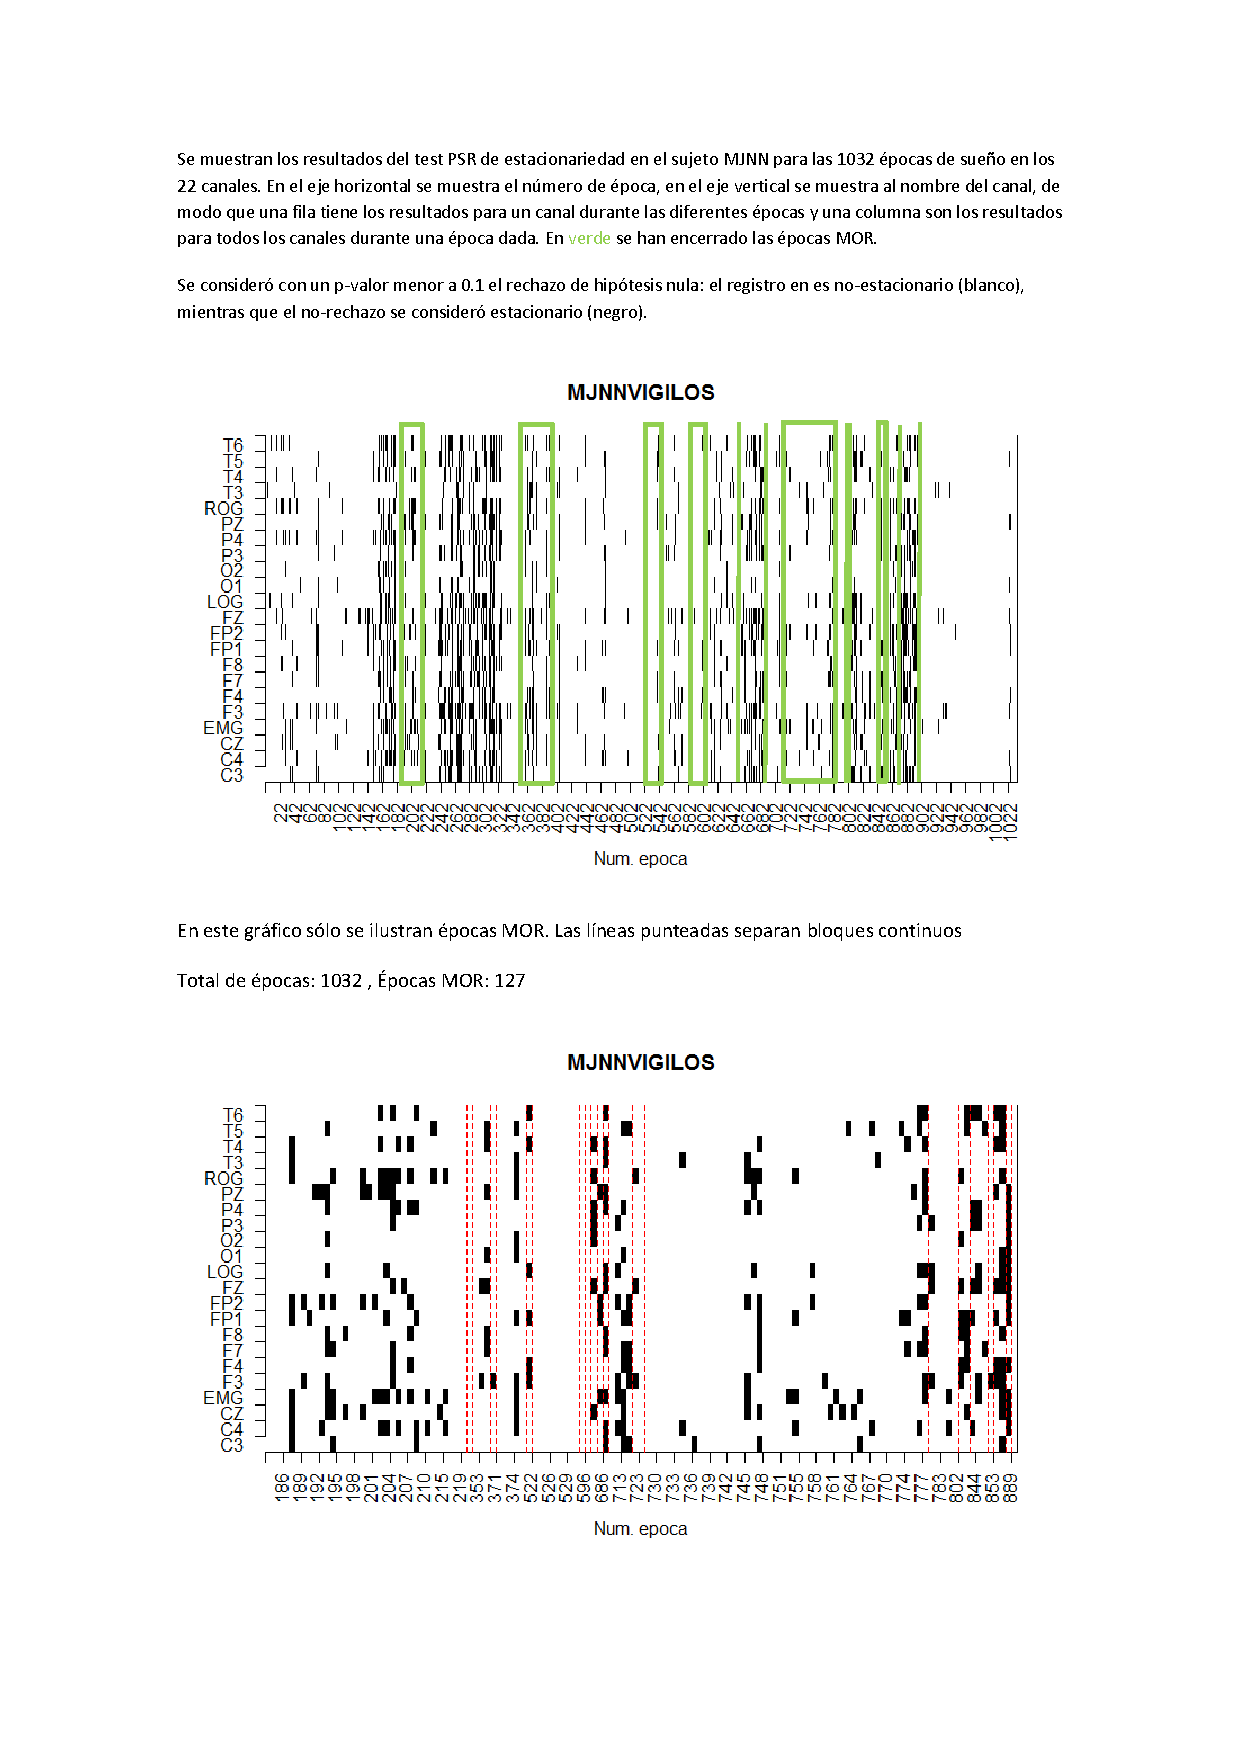
\includepdf[pages={1-},scale=.85]{reporte_de_estacionariedad_170120.pdf}
%%%%%%%%%%%%%%%%%%%%%%%%%%%%%%%%%%%%%%%%%%%%%%%%%%%%%%%%%%%%%%%%%%%%%%%%%%%%%%%%%%%%%%%%%%%%%%%%%%%
%%%%%%%%%%%%%%%%%%%%%%%%%%%%%%%%%%%%%%%%%%%%%%%%%%%%%%%%%%%%%%%%%%%%%%%%%%%%%%%%%%%%%%%%%%%%%%%%%%%